\paragraph{Western Bias in Wikidata}

Western bias analysis in Wikidata will be performed on 5 Wikidata classes: computer scientist, singer, memorial, university, and river. For each class, we collect the data for the western portion from 8 countries: Canada, France, Germany, Ireland, Poland, Switzerland, the United Kingdom (UK), and the United State of America (USA). For the non-western portion, we also chose 8 countries: China, Egypt, India, Indonesia, Japan, Morocco, Nigeria, and South Africa.

To analyze the bias, the first aspect that will be considered is the proportion of each regional category in every class. We assume that there are equal numbers of western and non-western and this will be the basis to determine if there is any bias in the data. Pearson's chi-square test (goodness-of-fit) is then performed to test the null and alternative hypotheses with significance level of \(\alpha=5\%\) as follows:

\(H_0\): The proportions of western and non-western entities in a particular class are equal

\(H_1\): The proportions of western and non-western entities in a particular class are not equal


\begin{center}
\small
\begin{threeparttable}
\caption{Entity Count of 5 Wikidata Classes per Regional Category}
\label{tab:western - entity count}
\begin{tabular}{c | c c c c c c c} 

\toprule
    Class Name & Entity & Western & \CellWithForceBreak{Non- \\ western} & \%Western & \CellWithForceBreak{\%Non- \\ western}& $\chi$^2 & p-value \\ [0.5ex] 
\midrule
    Computer scientist & 6063 & 5446 & 617 & 0.90 & 0.10 & 3846.15 & 0.0 \\
    Singer & 43240 & 31039 & 12201 & 0.72 & 0.28 & 8206.99 & 0.0 \\
    Memorial & 4011 & 3836 & 175 & 0.96 & 0.04 & 3341.54 & 0.0 \\
    University & 6124 & 2398 & 3726 & 0.39 & 0.61 & 287.98 & 1.37e-64 \\
    River & 125567 & 70059 & 55508 & 0.56 & 0.44 & 1686.20 & 0.0 \\
    [1ex]
\bottomrule
\end{tabular}
\begin{tablenotes}
    \footnotesize
    This table shows the entity count of 5 Wikidata classes per regional category. Chi-square test result shows the significance of difference between the entity count of the two genders male and female.
\end{tablenotes}
\end{threeparttable}
\end{center}

In terms of entity count, \autoref{tab:western - entity count} shows that there are big gaps between the westerners and non-westerners in all of the classes. From \autoref{tab:western - central tendency}, non-western entities generally have lower values of measure of central tendency (mean, median, mode). The range of property count of non-westerns is generally also lower than the westerns. Positive values of skewness (skewness > 0) and high kurtosis values (kurtosis > 3) in all classes denote the wealth distribution is right skewed and leptokurtic.

\begin{center}
\small
\begin{threeparttable}
\caption{Measures of Central Tendency of 5 Wikidata Classes per Regional Category}
\label{tab:western - central tendency}
\begin{tabular}{c | c c c} 
\toprule
    Class Name & \CellWithForceBreak{Mean \\ (o/w/n)} & \CellWithForceBreak{Median \\ (o/w/n)} & \CellWithForceBreak{Mode \\ (o/w/n)} \\ [0.5ex] 
\midrule
    Computer scientist & 35.00/35.87/27.24 & 29.00/29.00/22.00 & 21/15/16 \\
    Singer & 34.99/39.14/24.43 & 25.00/29.00/18.00 & 15/18/14 \\
    Memorial & 11.04/11.04/11.13 & 9.00/9.00/9.00 & 9/9/9 \\
    University & 23.11/31.61/17.63 & 17.50/24.00/16.00 & 6/6/6 \\
    River & 7.69/8.55/6.60 & 7.00/7.00/6.00 & 7/7/7 \\
    [1ex]
\bottomrule
\end{tabular}
\begin{tablenotes}
    \footnotesize
    This table shows the measures of central tendency of 5 Wikidata classes per regional category. Each measure will have 3 values: o (overall), w (western), and f (non-western).
\end{tablenotes}
\end{threeparttable}
\end{center}

\begin{center}
\small
\begin{threeparttable}
\caption{Measures of Dispersion and Symmetry of 5 Wikidata Classes per Gender Category}
\label{tab:western - dispersion and symmetry}
\begin{tabular}{c | c c c c c} 

\toprule
    Class Name & \CellWithForceBreak{Min \\ (o/w/n)} & \CellWithForceBreak{Max \\ (o/w/n)} & \CellWithForceBreak{Std. Deviation \\ (o/w/n)} & \CellWithForceBreak{Skewness \\ (o/w/n)} & \CellWithForceBreak{Kurtosis \\ (o/w/n)} \\ [0.5ex] 
\midrule
    Computer scientist & 4/4/5 & 441/441/145 & 25.15/25.67/18.15 & 3.02/3.02/2.37 & 20.90/20.83/8.49 \\
    Singer & 3/4/3 & 687/687/379 & 33.27/36.60/18.94 & 4.49/4.28/3.15 & 35.56/31.09/21.59 \\
    Memorial & 2/3/2 & 142/142/52 & 5.89/5.82/7.28 & 8.50/8.95/2.98 & 143.57/156.15/12.79 \\
    University & 2/2/2 & 234/234/166 & 20.00/25.88/12.25 & 2.37/1.65/2.22 & 10.34/5.33/12.70 \\
    River & 2/2/2 & 452/452/148 & 5.24/6.46/2.68 & 21.71/19.54/14.67 & 1152.84/868.56/465.42 \\
    [1ex]
\bottomrule
\end{tabular}
\begin{tablenotes}
    \footnotesize
    This table shows the measures of dispersion and symmetry of 5 Wikidata classes per gender category. Each measure will have 3 values: o (overall), w (western), and f (non-western).
\end{tablenotes}
\end{threeparttable}
\end{center}

Out of 5 classes, class of memorial is the only class where the null hypothesis is not rejected. In the other 4 classes, we can see a significant difference between the mean of the two reginal categories, which all are in favor of the western.

\begin{center}
\small
\begin{threeparttable}
\caption{F-Test, T-Test, and Welch's Test Result of 5 Wikidata Classes}
\label{tab:western - mean test}
\begin{tabular}{c | c c c c c c} 
\toprule
    Class Name & \CellWithForceBreak{F-Test \\ statistic} & \CellWithForceBreak{F-Test \\ p-value} & \CellWithForceBreak{T-Test \\ statistic} & \CellWithForceBreak{T-Test \\ p-value} & \CellWithForceBreak{Welch's Test \\ statistic} & \CellWithForceBreak{Welch's \\ p-value} \\ [0.5ex] 
\midrule
    Computer scientist & 2.00 & 1.00 & 8.13 & 5.10e-16 & 10.66 & 3.64e-25 \\
    Singer & 3.73 & 1.00 & 42.22 & 0.0 & 54.59 & 0.0 \\
    Memorial & 0.64 & 0.00 & -0.19 & 0.85 & -0.16 & 0.88 \\
    University & 4.46 & 1.00 & 28.40 & 8.23e-167 & 24.73 & 2.12e-123 \\
    River & 5.83 & 1.00 & 66.91 & 0.0 & 72.64 & 0.0 \\
 [1ex]
\bottomrule
\end{tabular}
\begin{tablenotes}
    \footnotesize
\end{tablenotes}
\end{threeparttable}
\end{center}

\begin{figure}[htp]
\centering 
\subfloat[Ratio of Class Wealth to Expectation per Cumulative Top Percentage - All Classes Average
\label{fig:test1 - western}]{%
  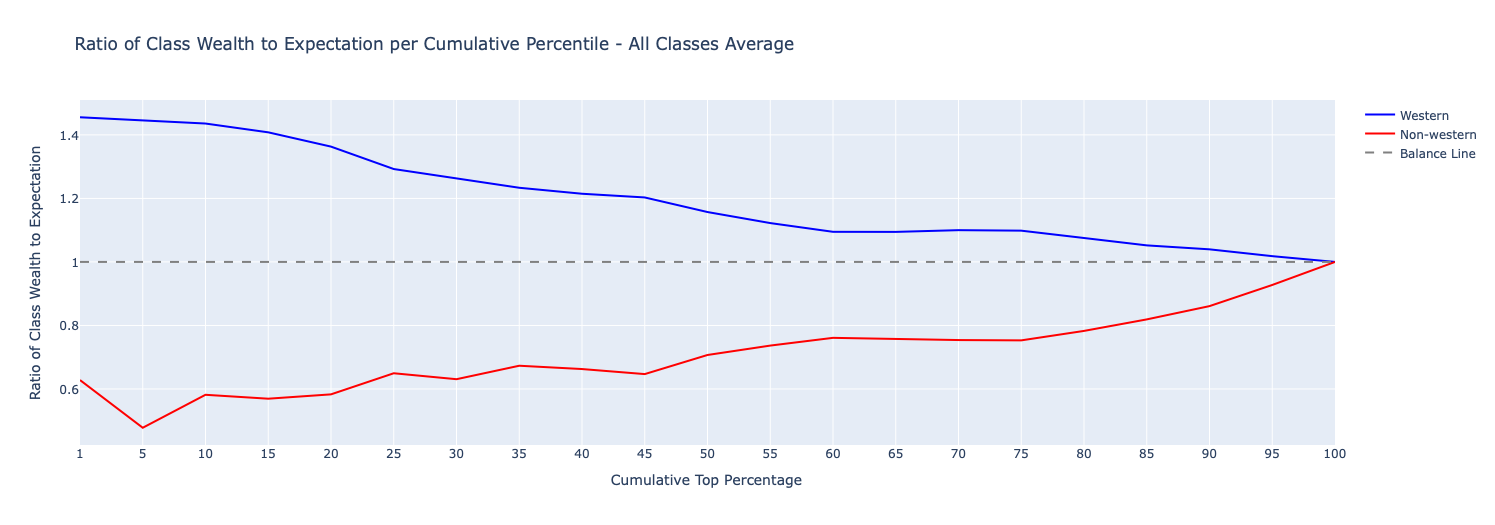
\includegraphics[clip,width=1.0\columnwidth]{Ratio of Class Wealth to Expectation per Cumulative Top Percentage - All Classes Average - Region}%
}

\subfloat[Ratio of Class Wealth to Expectation per Quantile - All Classes Average\label{fig:test2 - western}]{%
  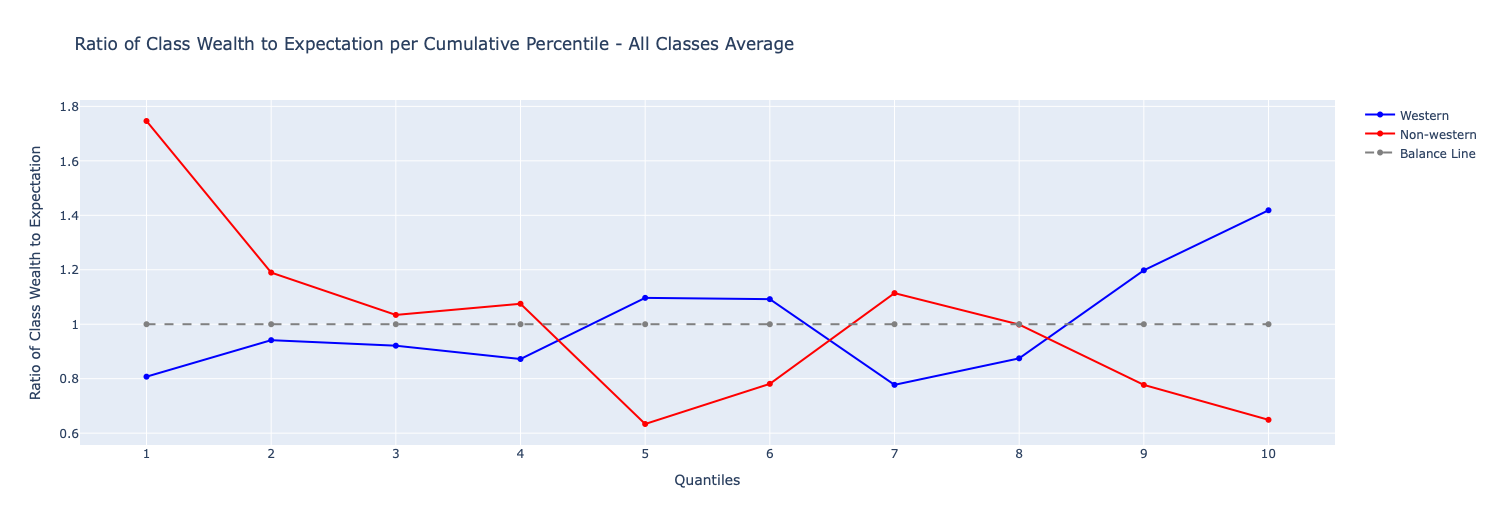
\includegraphics[clip,width=1.0\columnwidth]{Ratio of Class Wealth to Expectation per Quantile - All Classes Average - Gender - Region}%
}

\caption{...}
\label{fig:western - ratio of regional wealth to expectation}

\end{figure}